\documentclass[a4paper]{article}
\usepackage{graphicx} %Required for diagrams
\usepackage[bookmarks=true]{hyperref}
\usepackage{bookmark}%Required to do pdf bookmarking
\usepackage{booktabs}
\usepackage[margin=1.2in]{geometry}
\usepackage{float}
\usepackage{caption}
\usepackage{hyperref}%Required for referencing website pages
\usepackage[english]{babel}

\usepackage{graphicx}
\usepackage{dcolumn}
\usepackage[table]{xcolor}

\title{Burn Down And Velocity Char}
\author{Baobab Team}

\begin{document}
\newpage

\begin{titlepage}

\begin{center}


\includegraphics[width=400px]{pictures/logo.jpg}
\vspace{0.5 cm}
\begin{flushright} \large
\begin{tabular}{lr}
\vspace{1 cm}
\LARGE\textbf{Document:}Sprint Report 6\\

\vspace{1 cm}
\LARGE\textbf{Project:} Group Chat For Linphone (Agile DO-178)\\
\vspace{1 cm}
\LARGE\textbf{Advisor:} Kobus Coetzee\\
\vspace{1 cm}
\LARGE\textbf{Sponsors:} Nanoteq \& Department of Computer Science, UP\\
\vspace{1 cm}
\LARGE\textbf{Date: }\today\\
\end{tabular}
\end{flushright}

\centering 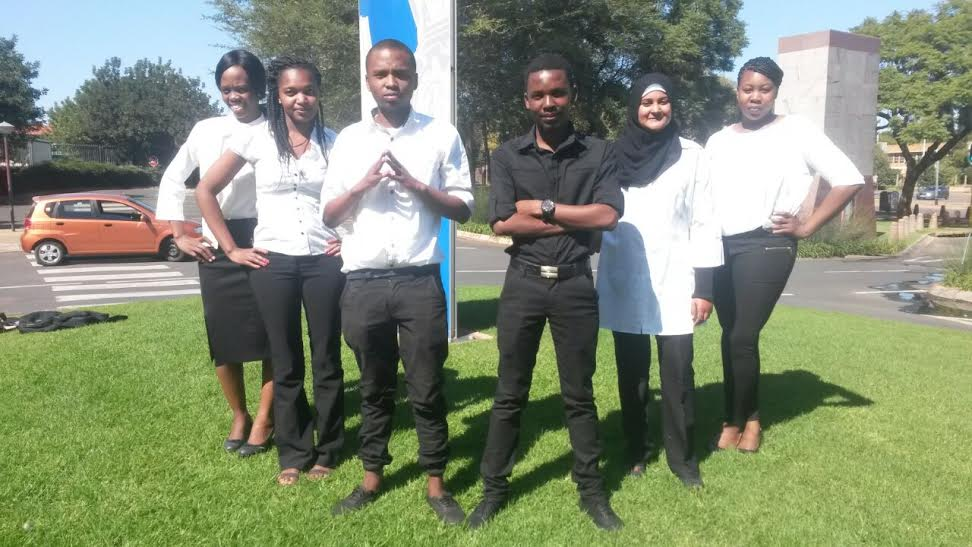
\includegraphics[width=350px]{pictures/Team.jpg}

Patience Mtsweni, Lerato Molokomme, Tsepo Ntsaba, Mpedi Mello, Lutfiyya Razak, Ephiphania Munava\\


\end{center}
\end{titlepage}
\newpage

\section{Introduction}
Software Accomplishment Summary is a list of all requirements that we have completed within the project.

\vspace{\baselineskip}

\section{Task Description}
\vspace{\baselineskip}
\begin{table} [H] 
\begin{tabular}{p{3cm} p{3cm} p{3.5cm} p{1cm}} 
\hline %\toprule % Top horizontal line
&&&\\
\textbf{Story Name} & \textbf{Task Number} & \textbf{Task Description} & \textbf{Status}\\ % Column names row
&&&\\
\hline

 & 1 & Linux & Done\\ \cmidrule(l){2-4}

 & 2 & Eclipse & Done\\ \cmidrule(l){2-4}

 & 3 & Android SDK & Done \\ \cmidrule(l){2-4}
 
 Environment Setup & 4 & Android NDK & Done \\ \cmidrule(l){2-4}

 & 5 & Android eclipse ADT & Done\\ \cmidrule(l){2-4}

 & 6 & C Compiler & Done\\ \cmidrule(l){2-4}
 
 & 7 & Clone Linphone project recursive & Done \\ \cmidrule(l){2-4}

 & 8 &  Compile project  & Done \\  
\midrule % In-table horizontal line

 Setup CI Travis & 9 & YAML File & Done \\ \cmidrule(l){2-4}

 & 10 & Python File & Done \\  
 Setup CD & 11 & Devices Deployment & Done \\
\midrule

Group Chat Interface & 12 & Activity for Each Screen & Done\\ \cmidrule(l){2-4}

& 13 & Group Chat functionality Icons & Done\\ 
\midrule

Select Participants & 14 & List Member User-names & Done \\ \cmidrule(l){2-4}



 & 15 & List Member SIP Addresses & Done \\ 
\midrule

& 16 & About Button & Done \\ \cmidrule(l){2-4}

Welcome Screen & 17 & Help Button & Done\\ \cmidrule(l){2-4}

& 18 & Logo & Done\\ 
\midrule

 & 19 & Group name & Done\\\cmidrule(l){2-4}


Select Group Details &  20  & Group icon & Done\\\cmidrule(l){2-4}

 & 21 & Exit group icon & Done\\\cmidrule(l){2-4}

 & 22 & Add participants & Done\\ 
 \midrule

Type Message & 23 & Type Message & Done\\ 
 \midrule
 
 Send Message & 24 & Send Message & Done\\ 
\hline
\end{tabular}
\caption{Task 1} % Table caption, can be commented out if no caption is required
\label{tab:template} % A label for referencing this table elsewhere, references are used in text as \ref{label}
\end{table}

\pagebreak
 
\begin{table} [H] 
\begin{tabular}{p{3cm} p{3cm} p{3.5cm} p{1cm}} 
\hline %\toprule % Top horizontal line
&&&\\
\textbf{Story Name} & \textbf{Task Number} & \textbf{Task Description} & \textbf{Status}\\ % Column names row
&&&\\
\hline

 
 Receive Message & 25 & Receive Message & Done\\ 
 \midrule
 
 Record Voice & 26 & Record Voice & Done\\ 
\midrule

  Send Encrypted Group Messages & 29 & Send Encrypted Group Messages & Done\\ 
 \midrule
 
 Receive Encrypted Group Messages & 30 & Receive Encrypted Group Messages & Done\\ 
 \midrule

 
  Send Encrypted Pictures & 29 & Send Encrypted Group Messages & Done\\ 
 \midrule
 
 Receive Encrypted Pictures & 30 & Receive Encrypted Group Messages & Done\\ 
\hline

\end{tabular}
\caption{Task 2} % Table caption, can be commented out if no caption is required
\label{tab:template} % A label for referencing this table elsewhere, references are used in text as \ref{label}
\end{table}
\end{document}

